% !TeX spellcheck = en_GB
\documentclass[]{article}

\usepackage[style=apa, backend=biber, sorting=ynt, sortcites=true, useprefix=true]{biblatex}
\usepackage[autostyle=false, style=english]{csquotes}
	\MakeOuterQuote{"}
\usepackage[british]{babel}
\usepackage[modulo]{lineno}
\linenumbers

\usepackage{booktabs}

\usepackage{amsmath}
\usepackage{enumitem}


\usepackage{graphicx}
\usepackage{subcaption}

\usepackage{etoolbox}

\usepackage[hidelinks]{hyperref}

\usepackage{appendix}

\AtBeginEnvironment{tabular}{\small}


\addbibresource{thesis.bib}

\title{An AB-SFC insight on the macroeconomic effects of an UBI}
\author{Margherita Redigonda}
\date{}


\begin{document}

\maketitle

\begin{abstract}
    The paper tries to answer the question "How can the macroeconomic effect of an Universal Basic Income (UBI) be studied?".
    It adopts an Agent Based - Stock Flow Consistent approach to address the problem, developing a model rooted in the real side of the economy with endogenous heterogeneity in wealth and wages.
    It shows that an UBI increases the private demand and the inequality in the system, but that introducing keynesian taxation-based policy counteracts the inequality effect with only minor effects on the demand side.

Keywords : AB-SFC; UBI; taxation

JEL Codes: E12, E24, E27
\end{abstract}

\section{Why an Agent-Based Model?}
\label{ch:why}
The paper tries to answer the question "How can the macroeconomic effect of an Universal Basic Income (UBI) be studied?".

To follow a complex approach \parencite{Redigonda2023}, we have to find which scales are relevant and which levels on them are the most suitable to study the phenomenon.

The aggregation scale it is certainly to be taken in account: an UBI is essentially a microeconomic policy, or at least it affects individual behaviour, while we want to observe the aggregate effects (i.e. inflation, growth, ...) of such policy.

Generally speaking, every time we want to address inequalities in a model we cannot consider only the most aggregate level of representation.

Post-Keynesian tradition usually adopts a class perspective with a Kaleckian approximation in which people are split in two classes: capitalists, who do not work and only receive dividends, and workers, who receive wages but not dividends.
This approach is very simple and is already able to produce sound economic theory, but it is possible to point at two big shortcomings.
First, it is not possible to measure a fine-grained inequality index à la Gini, but only something like a Top10 Bottom90 ratio à la Piketty-Zuckman-Saez \parencite{piketty2003, piketty2014}.
Second, as noted by, for example, Piketty nowadays it is very common to have mixed sources of income both in the lower strata (e.g. pension founds are based on dividends and financial income) and upper strata (CEO and top manager usually have a mix of stocks with dividends and wages as income sources).

We can refine the descriptiveness of the model by increasing the number of subdivisions of people, and allowing for mixed income sources for each subdivision.
But as the number of subdivisions grows it becomes more and more difficult to find elegant solutions for the model and practically impossible to find analytical ones.
Actually, it becomes necessary to adopt a computational approach \parencite{tesfatsion2006a} and when the number of subdivisions grows enough, each subdivision can be interpreted no longer as a class but rather as a single person, which can be described by microeconomic theory.
This line of thinking leads to what in literature is known as Agent-Based Models \parencite{arthur2021, farmer2012} and allows to create a bridge between macroeconomics and microeconomics without the need of a representative agent \parencite{dosi2019}.
A similar argument can be held for firms: instead of representing them as a single homogenous sector, it is possible to introduce in the model a plurality of agents each representing a different (group of) firm(s) with different technology, strategy or wage level, allowing representing competition and innovation among firms.

Another framework significant to adopt are the Stock-Flow Consistent models \parencite{nikiforos2017,godley2012}: this class of models recognizes that any monetary or financial flow in the economy leave behind a credit and a corresponding debt, that financial wealth cannot be created but only transferred (with public debt as primary source of it).
This is relevant if we are focusing on distributional effects and inequalities: those models make impossible to increase the (financial) wealth of someone without making someone else poorer at the same time, preventing the possibility to create an ad hoc model in which wealth accumulation is a positive sum process.

These two ideas have been already put together generating a rich stream of papers collectively known as AB-SFC models \parencite{caverzasi2018}, with some of them able to reproduce a significant number of economic theory results and economic empirical observation in simulations with a high agent count \parencite[e.g.][]{caiani2016,reissl2024,dawid2019,dosi2010}.
This synthesis does not prescribe a specific economics theory to model the behaviour of each agent and the general structure of the economy, but all the model cited above are grounded in post-Keynesian theory \parencite{lavoie2022}\footnote{The mainstream economics have developed the HANK models to address the problem of heterogeneity among agents \parencite{violante2021}, while for example an SFC model for Italian economy developed by the ministry of finance does not rely on a post-Keynesian closure \parencite{barbierihermitte2023}.}.
We chose to found the behavioural equations of the model mostly on post-Keynesian theory for its greater realism compared to the neoclassical microeconomic theory \parencite{kirman1992,arnsperger2006}.

The model developed in this paper focuses on production, based on the hypothesis that wages and innovation play a more significant role in differentiating the level of income than the financial side of the economy.

Capital goods are accounted for using discrete objects, in order to be matched with workers in a Leontief production function.
Clearly, this assumes that each worker is a full-time employee or that, equivalently, we account for the full-time equivalent number of employees: this is an approximation that straightlines the model, reducing heterogeneity where not strictly needed. 
This approach allows implementing capital goods as objects with different productivity levels, "skills" required to be used and wages associated, to enable differentiation in wages levels and firm-worker matches.
Such a choice of modelling allows for observing a continuous wage curve instead a segmented one, usually assuming a constant level of wage for each class of workers (e.g. low-, medium- and high-trained) \parencite{caiani2019b}\footnote{Some models as \textcite{dosi2021a} represent heterogeneous wages levels at the agent-level, but the resulting distribution is not reported.}.

Moreover, SFC models highlights that the financial side of the economy is only a matter of accounting, of societal norms and distribution of power.
Which is very relevant for many of the dynamics of a model, but it is not sufficient.
The economy at its core is a question of time (labour), matter and energy (natural resources); an idea often overlooked in Economics, focusing way more on Money than on Land and Labour using Polaniy's words.
The choice to root the model in the production side of the economy is also a way to recognize, highlight and follow this intuition.

The financial side is kept as simple as possible, assuming as a first approximation that the rent derived from wealth is proportional to the household's wealth.
While it is true that richer individuals are able to achieve higher return rate on their wealth, this mechanism only accelerates the increasing in inequality rather than creating it.

The attempt presented here is to develop a simple model that sketches an unequal distribution of income and wealth (ideally fat-tailed) rooted in the labour market dynamics, that can be later used as a baseline to compare different welfare policies, such as an UBI.

\section{The matrices of the model}

\begin{table}
    \centering
    \begin{tabular}{l|ccccc|l}
                 & $\mathcal{H}$             & $\mathcal{F}_\mathbf{C}$               & $\mathcal{F}_\mathbf{K}$               & $\mathcal{B}$    & $\mathcal{G}$    & $\Sigma$                   \\
        \midrule
        Money    & $+\mathbf{M}_\mathcal{H}$ & $+\mathbf{M}_{\mathcal{F}_\mathbf{C}}$ & $+\mathbf{M}_{\mathcal{F}_\mathbf{K}}$ & $-\mathbf{M}$    &                  & 0                          \\
        Loans    &                           & $-\mathbf{L}_{\mathcal{F}_\mathbf{C}}$ & $-\mathbf{L}_{\mathcal{F}_\mathbf{K}}$ & $+\mathbf{L}$    &                  & 0                          \\
        Bonds    &                           &                                        &                                        & $+\mathbf{B}$    & $-\mathbf{B}$    & 0                          \\
        \midrule
        Capital  &                           & $+p_\mathbf{K} \mathbf{K}_\mathbf{C}$  & $+p_\mathbf{K} \mathbf{K}_\mathbf{K}$  &                  &                  & $+p_\mathbf{K} \mathbf{K}$ \\
        \midrule
        $\Sigma$ & $+V_\mathcal{H}$          & $+V_{\mathcal{F}_\mathbf{C}}$          & $+V_{\mathcal{F}_\mathbf{K}}$          & $+V_\mathcal{B}$ & $+V_\mathcal{G}$ & $+p_\mathbf{K} \mathbf{K}$ \\
    \end{tabular}
    \caption{Balance sheet for the model with investments}
\end{table}

\begin{table}
    \centering
    \begin{tabular}{l|ccccc|l}

                               & $\mathcal{H}$                   & $\mathcal{F}_\mathbf{C}$                                                                                    & $\mathcal{F}_\mathbf{K}$                                                                                    & $\mathcal{B}$                                             & $\mathcal{G}$       & $\Sigma$ \\
        \midrule
        Consumption            & $-p C$                          & $+p C$                                                                                                      &                                                                                                             &                                                           &                     & 0        \\
        Gvt Spending           &                                 & $+p G$                                                                                                      &                                                                                                             &                                                           & $-p G$              & 0        \\
        Investments            &                                 & $-p_\mathbf{K} I_{\mathcal{F}_\mathbf{C}}$                                                                  & $+p_\mathbf{K} I_{\mathcal{F}_\mathbf{C}}$                                                                  &                                                           &                     & 0        \\
        Benefits               & $+UB$                           &                                                                                                             &                                                                                                             &                                                           & $-UB$               & 0        \\
        Wages                  & $+W$                            & $-W_{\mathcal{F}_\mathbf{C}}$                                                                               & $-W_{\mathcal{F}_\mathbf{K}}$                                                                               &                                                           &                     & 0        \\
        Profits                & $+P$                            & $-P_{\mathcal{F}_\mathbf{C}}$                                                                               & $-P_{\mathcal{F}_\mathbf{K}}$                                                                               & $-P_\mathcal{B}$                                          &                     & 0        \\
        Taxes                  &
        $-T$                   &                                 &                                                                                                             &                                                                                                             & $+T$                                                      & 0                              \\
        \midrule
        $\mathbf{L}$ interests &                                 & $-r_\mathbf{L} (\Delta^+\mathbf{L}_{\mathcal{F}_\mathbf{C}} + {\mathbf{L}_{\mathcal{F}_\mathbf{C}}}_{t-1})$ & $-r_\mathbf{L} (\Delta^+\mathbf{L}_{\mathcal{F}_\mathbf{K}} + {\mathbf{L}_{\mathcal{F}_\mathbf{K}}}_{t-1})$ & $+r_\mathbf{L} (\Delta^+\mathbf{L} + {\mathbf{L}}_{t-1})$ &                     & 0        \\
        $\mathbf{B}$ interests &
                               &                                 &                                                                                                             & $+r_\mathbf{B}\mathbf{B}$                                                                                   & $-r_\mathbf{B}\mathbf{B}$                                 & 0                              \\
        \midrule
        $\Delta$ Money         & $-\Delta\mathbf{M}_\mathcal{H}$ & $-\Delta\mathbf{M}_{\mathcal{F}_\mathbf{C}}$                                                                & $-\Delta\mathbf{M}_{\mathcal{F}_\mathbf{K}}$                                                                & $+\Delta\mathbf{M}$                                       &                     & 0        \\
        $\Delta$ Loans         &                                 & $+\Delta\mathbf{L}_{\mathcal{F}_\mathbf{C}}$                                                                & $+\Delta\mathbf{L}_{\mathcal{F}_\mathbf{K}}$                                                                & $-\Delta\mathbf{L}_{\mathcal{B}}$                         &                     & 0        \\
        $\Delta$ Bonds         &                                 &                                                                                                             &                                                                                                             & $-\Delta\mathbf{B}$                                       & $+\Delta\mathbf{B}$ & 0        \\
        \midrule
        $\Sigma$               & 0                               & 0                                                                                                           & 0                                                                                                           & 0                                                         & 0                   & 0        \\
    \end{tabular}
    \caption{Transactions and Flows matrix for the model with investments}
\end{table}

The design of an SFC starts from the accounting matrices. The model includes five sectors, three that are composed by agents (Households, Consumption Firms, Capital Firms) and two aggregate one (the financial one denoted with $\mathcal{B}$ as Bank, and the aggregate public sector denoted with $\mathcal{G}$ as Government).

In the balance sheet matrix we see four different assets: Money issued by the financial sector and used by households and firms; Loans issued by the financial sector in favour of the Firms with the relative interests; Government Bonds used by the financial sector as both reserves and advances with the relative interests; and the productive Capital owned by the Firms.

The Flows of Founds matrix is quite standard, with the only unusual entry is the unemployment benefits.

\section{The Behavioural Equations}
Prices (p) are determined by a cost plus mark-up strategy like $$p = (1 + \mu) \frac{W_{TOT}}{Y}$$ where Y is the total output and $\mu$ is the mark-up rate.
By employing a Leontief production function the production ($\beta$) is the ratio between the single input and the output, and so prices can also be written as $$p= (1+\mu) <W> <\beta>$$

The mark-up is updated by each sector looking at its own capacity utilization like $$\mu = \mu_{t-1} (1 + \Theta_{\mu} \frac{{cu}_{t-1} - {cu}^T}{{cu}^T})$$ where $\Theta_{\mu}$ regulates the speed of the adjustment.

Unemployment benefits (UB) are an exogenous and constant fraction $\phi$ of the average wage.

Workers' skills are updated asymmetrically as 
$$\sigma_{t-1} = \sigma (1+\frac{\delta_\sigma}{D})$$
if the worker is employed (where D is a deflator of the dynamics and $\delta_\sigma$ is the rate of variation), and
$$\sigma_{t-1} = \max(1,\sigma / (1+\delta_\sigma))$$ if they is unemployed.

The modelling of the wage dynamics relies on the mismatch between the demand and the supply of labour: a higher unsatisfied demand leads to a faster wage growth.
The wages are update sector by sector as $$W_0 =  {W_0}_{t-1} (1 + \Theta_W \frac{N^T_{t-1} - N_{t-1}}{N^T_{t-1}})$$ where $W_0$ is the individual firm-proposed wage and $W = W_0 \sigma$ is the individual wage.

The behavioural equation chosen does not include the possibility that the nominal wages decrease, which is an acceptable approximation given that the most relevant mechanism of loss of purchase power is the reduction in the real wages caused by the inflation rather than the reduction of the nominal ones.

Taxes (T) are paid with a flat rate on wages ($\tau_W$), distributed profits ($\tau_P$) and consumption ($\tau_C$).

Desired consumption in units of good for households is defined in a classic post-Keynesian way as $$C^T = \frac{a_Y ((1 - \tau_W) W + UB) + a_V {\mathbf{M}_\mathcal{H}}_{t-1}}{(1 + \tau_C) <p_{t-1}>}$$
where $a_Y$ and $a_V$ are the marginal propensity to consume out of disposable income (wages and unemployment benefits) and wealth (money, $\mathbf{M}_\mathcal{H}$).
Additionally, at the denominator appears $(1 + \tau_C) <p_{t-1}>$ which is the price of the good for the consumers (including VAT) and allows converting the desired expenditures for consumption into the desired units of goods.

Government's desired consumption is determined against target expected deficit $d$ $$G^T = \frac{d \cdot {GDP}_{t-1} + T_{t-1} - UB_{t-1}}{<p_{t-1}>}$$

Given the desired total production $Y^T = (1+\rho_C)Y_{t-1}$, firms aim to hire a number of workers equal to $N = Y^T/<\beta>$.

Desired investments (in units of capital goods) are determined as $$I^T = {\mathbf{K}^u}_{t-1} (\frac{1}{{cu}^T} - \frac{1}{{cu}}) + \delta_\mathbf{K} \mathbf{K}_{t-1}$$ where $\mathbf{K}^u$ is the number of capital good matched by a worker in production and $cu$ and ${cu}^T$ are the capacity utilization rate of capital and its target value.

Firms receive loans from the bank to cover for wages and investment $$\Delta^+ \mathbf{L}_{\mathcal{F}_\mathbf{C}} = W_{\mathcal{F}_\mathbf{C}} + p_\mathbf{K} I_{\mathcal{F}_\mathbf{C}}$$ $$\Delta^+\mathbf{L}_{\mathcal{F}_\mathbf{K}} = W_{\mathcal{F}_\mathbf{K}}$$
At the end of the period the stock of money of the previous period and the income of the current one are used to repay the loans $$\mathbf{L}_{\mathcal{F}_\mathbf{C}} = {\mathbf{L}_{\mathcal{F}_\mathbf{C}}}_{t-1} + \Delta^+\mathbf{L}_{\mathcal{F}_\mathbf{C}} - {\mathbf{M}_{\mathcal{F}_\mathbf{C}}} - p_\mathbf{C} (C + G)$$ $$\mathbf{L}_{\mathcal{F}_\mathbf{K}} = {\mathbf{L}_{\mathcal{F}_\mathbf{K}}}_{t-1} + \Delta^+\mathbf{L}_{\mathcal{F}_\mathbf{K}} - {\mathbf{M}_{\mathcal{F}_\mathbf{K}}} - p_\mathbf{K} I_{\mathcal{F}_\mathbf{C}}$$

Then interest are paid on maximum amount of loans inside the period $\mathbf{L}_{t-1} + \Delta^+\mathbf{L}$

Firms aim to a null stock of money at the end of each period, so after having "closed the circuit", i.e. repaid the loans with the earnings of the period, they distribute any remaining wealth to households, proportionally to the wealth held by each household.

Bonds are issued by the government to finance the deficit and interests are paid on them; the accounting at the end of the period is $$\mathbf{B} = \frac{\mathbf{B}_{t-1} - (T - p_\mathbf{C}G - UB)}{1-r_\mathbf{B}}$$
where $r$ denotes the interest rate.

The interest rate on bond is determined with a Taylor-like rule depending on inflation ($i$), unemployment ($u$) and the capacity utilization as $$r_\mathbf{B} = i_{t-1} + \alpha_i (i_{i-1} - i^T) + \alpha_{cu} ({cu}_{t-1} - {cu}^T) - \alpha_u (u_{t-1} - u^T)$$ and the interest rate on loan is determined as a fixed premium on the interest rate on bonds.

The bank aims to keep a target wealth to loan ratio, which leads to the equation for the distributed profits (see appendix \ref{app:eq}) $$ P_\mathcal{B}  = \frac{1-r_\mathbf{B}}{1-r_\mathbf{B}+r_\mathbf{B}\tau_P}(\mathbf{V}_{t-1} - {cr}^T \mathbf{L} + r_\mathbf{L} (\Delta^+\mathbf{L} + \mathbf{L}_{t-1}) + \frac{r_\mathbf{B}}{1-r_\mathbf{B}}(\mathbf{B}_{t-1} + p_\mathbf{C} G + UB - \tau_C C - \tau_W W - \tau_P (P_{\mathcal{F}_\mathbf{C}} + P_{\mathcal{F}_\mathbf{K}})))$$
also distrubuted to the households proportionally to their wealth.

The last feature added to the model is a very simple innovation dynamics, which involves both the capital firms (which increase the productivity of their produced capital) and the workers (which accumulate "skills" ($\sigma$) to be able to used more advanced -i.e. productive- capital goods).

Innovation is modeled as an increase in the productivity of capital goods produced by capital firms. It is assumed to rise with the average skill level of employees (used as a proxy for human capital) and with market share, and to decline with firm age, as:
$$\beta = \beta_{t-1} + \iota_1 <\sigma> + \iota_2 \frac{p_\mathbf{K}I_{\mathcal{F}_\mathbf{C}}}{\Sigma p_\mathbf{K}I_{\mathcal{F}_\mathbf{C}}} - \iota_3 age$$


\section{The Event's List}
\begin{enumerate}[label=\textbf{\Alph*}]
    \item Households determinate the desired consumption (expressed as units of good) based on the wealth and the disposable income of the previous period
    \item Government determinate the desired consumption (expressed as units of good) based on the target deficit computed on the accounting of the previous period
    \item Investments are ordered by the consumption firms to the capital ones
    \item Firms fire and hire workers in order to match the labour input required to match the desired consumption
    \item The realized output is determined for both capital and consumption goods
    \item Wages and unemployment benefits are paid
    \item Prices are set
    \item Consumption goods are sold to households and the government
    \item Capital goods are sold to consumption firms
    \item Loans are written down to cover wages and investments
    \item Loans are repaid in their principal and interests
    \item Profits are distributed
    \item Taxes are paid
    \item Accounting variables are updated, including government bonds' interest
\end{enumerate}

\section{The (missing) calibration}
An open problem among researchers who develop (AB-)SFC models is the calibration of the model, i.e. finding the right values for the parameters to make the model fitting data or at least stylized facts \parencite{fagiolo2019a, grazzini2017a, zezza2019}.
The idea behind it is to increase the realism (and so the reliability) of the predictions. But as discussed in a wide literature about (neoclassical) economics, realism is not always a necessary requirement neither is a feature of models required in Economics today.
As such it is possible to remain inside the stylemes of the discipline without achieve a "quantitative realism", a mathematical model that fit accurately the real-world data, but rather to use mathematical models as a way to streamline and clarify complex thoughts, achieving a "qualitative realism" that match the general dynamics observed without looking at the exact figures (as in the spirits of many models of the XX\textsuperscript{th} century, even from the post-Keynesian school).

Additionally, SFC models are generally non-linear, with exponential or conditional dynamics (plus the effects of discretization if we consider the AB ones), which leads to chaotic behaviours. I mean chaotic in the strict mathematical sense: a model that change significantly its behaviour for small variations of the initial conditions (or in our case of the parameters).
This characteristic makes calibration a very difficult exercise that has to rely on stochastic and often black-boxed algorithm to find the right parameters, because it is not possible to assume that the macroscopic behaviours targeted for the calibration change continuously even for small variations of the parameter(s) of interest (even not considering the interactions among them).

The model presented here is developed more as a theoretical and thinking tool, a way to show basic economic interactions related to the introduction of an UBI.
As such, parameters values are got from literature and when needed roughly tuned by hand to obtain stable and not too much unrealistic dynamics.

\section{The scenarios}
The base version of the model shows a stable behaviour and enough heterogeneity and distributional inequalities. It makes somehow suitable to sketch an answer to the original question: what will happen if an UBI will be introduced?

A simple experiment has been set up, creating six scenarios and ten repetition for each of them. The scenarios are:
\begin{enumerate}
    \item the baseline model.
    \item a model with increased profit taxation.
    \item a model with the introduction of a wealth tax paid at the end of each period.
    \item a model with an UBI, implemented as if the unemployment benefits from the previous models are paid regardless the employment status.
    \item a model with an UBI and a wealth tax.
    \item a model with an UBI and an increased profit tax.
\end{enumerate}

\section{Results}

\begin{figure}
    \centering
    \begin{subfigure}[t]{0.49\textwidth}
        \centering
        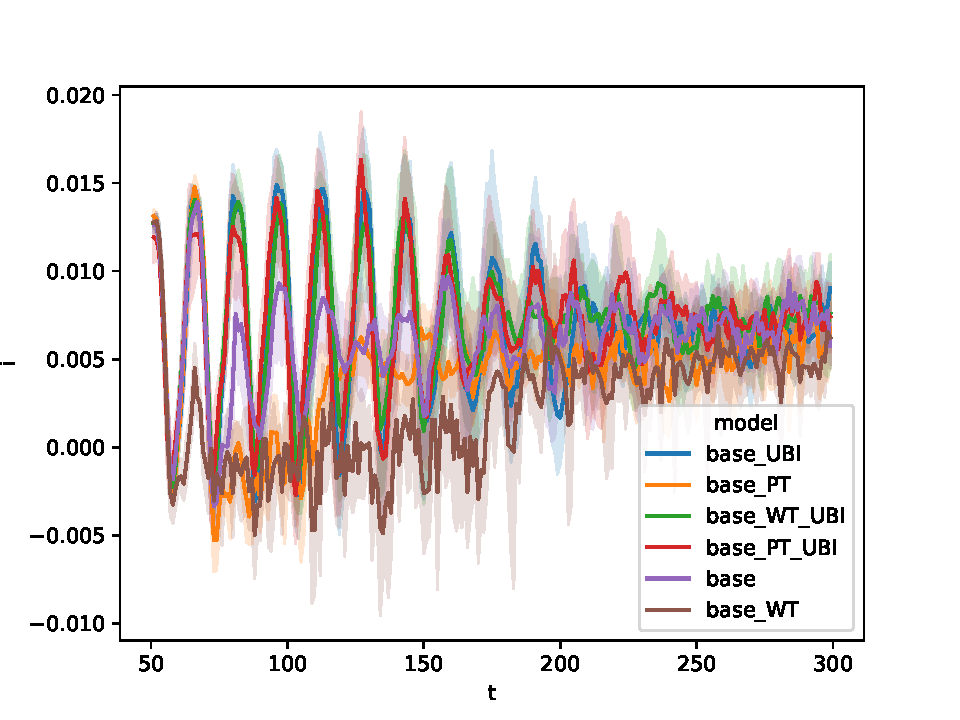
\includegraphics[width=\textwidth]{i}
        \caption{Dynamics of inflation after the first few periods}
        \label{fig:pol_i}
    \end{subfigure}%
    ~
    \begin{subfigure}[t]{0.49\textwidth}
        \centering
        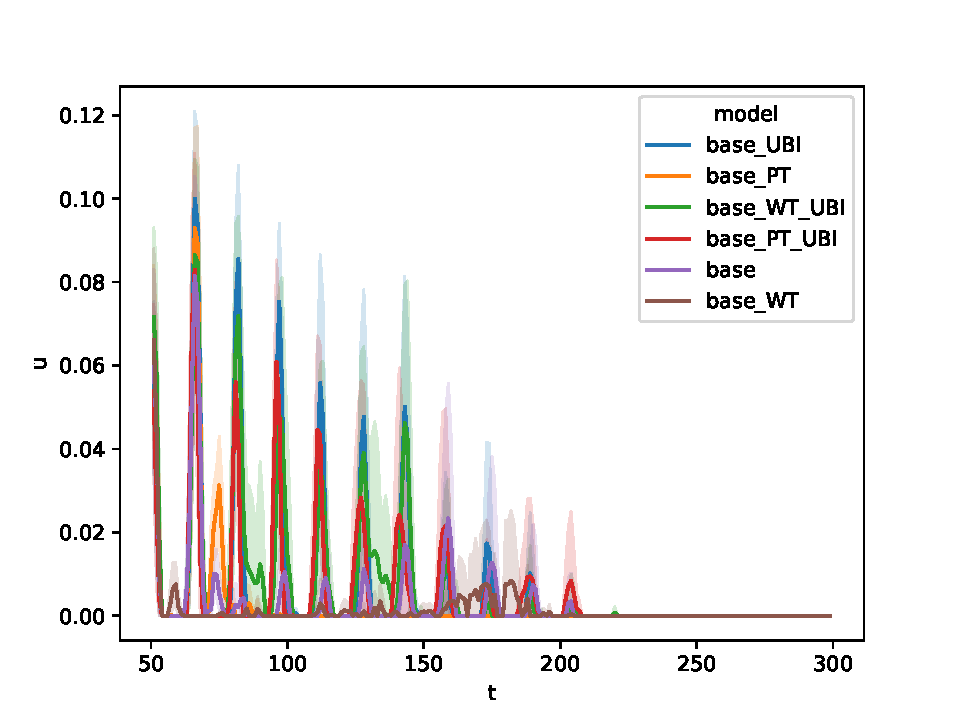
\includegraphics[width=\textwidth]{u}
        \caption{Dynamics of unemployment after the first few periods}
        \label{fig:pol_u}
    \end{subfigure}
    \begin{subfigure}[t]{0.49\textwidth}
        \centering
        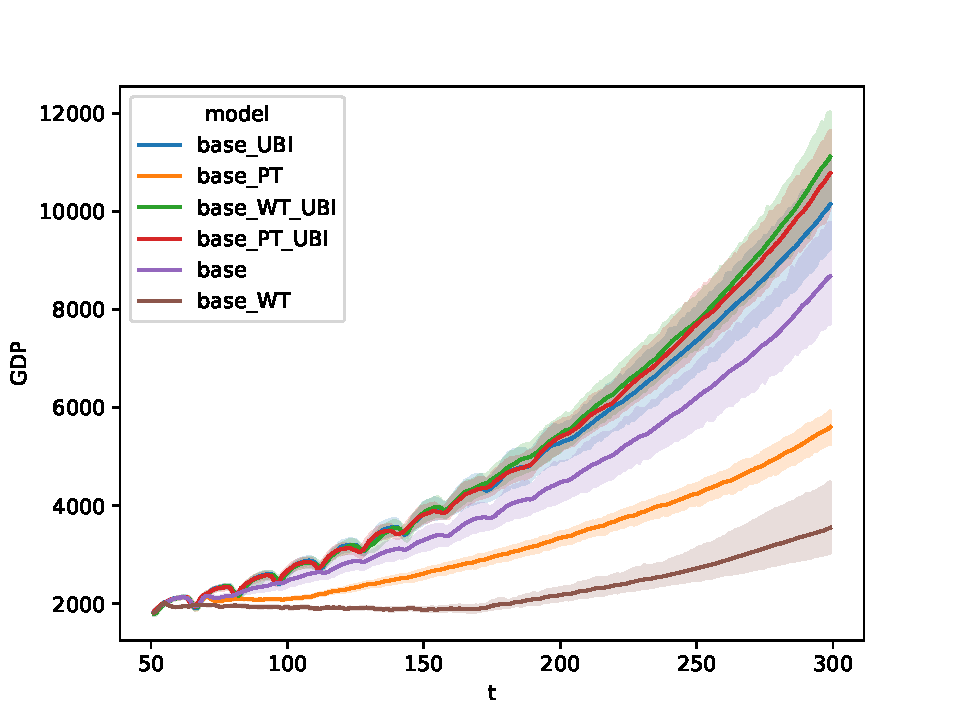
\includegraphics[width=\textwidth]{GDP}
        \caption{Dynamics of nominal GDP}
        \label{fig:pol_sb}
    \end{subfigure}%
    ~
    \begin{subfigure}[t]{0.49\textwidth}
        \centering
        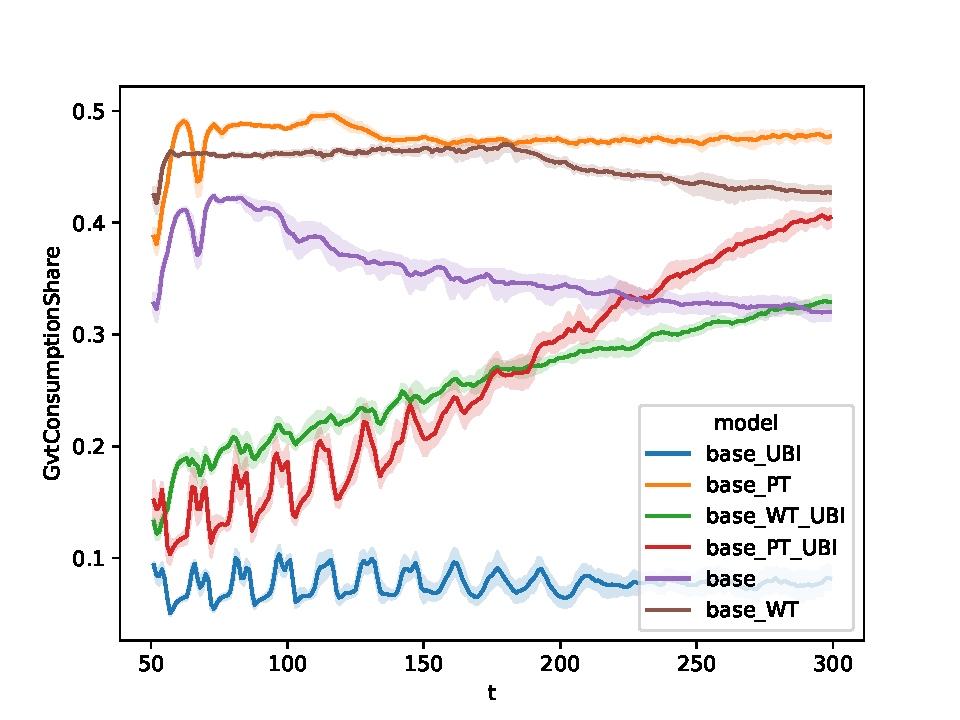
\includegraphics[width=\textwidth]{Gvt}
        \caption{Dynamics of the share of public consumption}
        \label{fig:pol_wd}
    \end{subfigure}
    \begin{subfigure}[t]{0.49\textwidth}
        \centering
        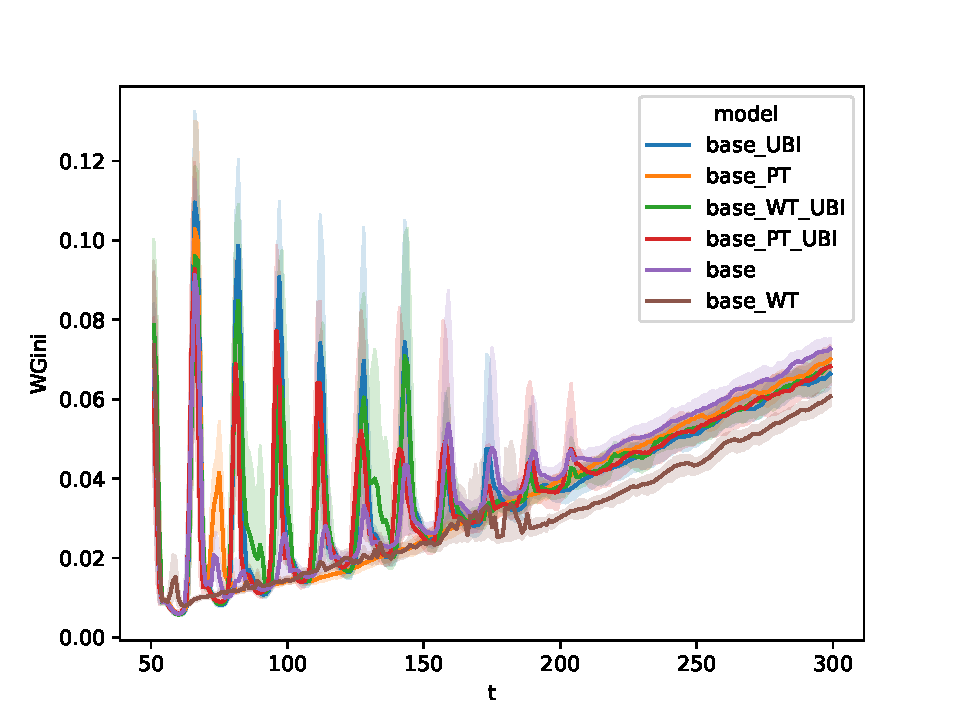
\includegraphics[width=\textwidth]{WGini}
        \caption{Dynamics of Gini index calculated on wages}
        \label{fig:pol_sdist}
    \end{subfigure}%
    ~
    \begin{subfigure}[t]{0.49\textwidth}
        \centering
        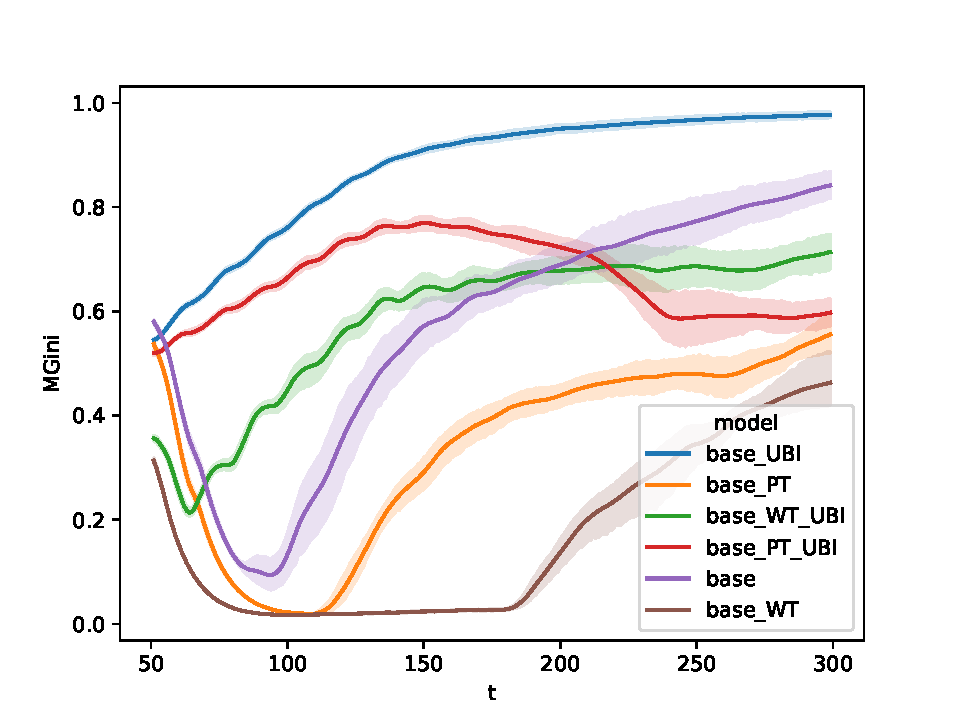
\includegraphics[width=\textwidth]{MGini}
        \caption{Dynamics of Gini index calculated on wealth after the first few periods}
        \label{fig:pol_bdist}
    \end{subfigure}
    \caption{Dynamics of the AB model with innovation}
\end{figure}

The emerging results are not necessarily intuitive.
The introduction of an UBI accelerates the nominal growth of the model, its instability and move consumption from the public to the private sector.
But at the same time it is the policy that most increase the Gini index, appearing as the policy less able to reduce inequalities.
This is reasonably because such a policy sustains the demand through a direct transfer of wealth from the public to the private sector, reducing the relative government consumption (which is not included in the Gini calculation) and increasing the private one.

Old Keynesian policies based on taxation slow down the economy but at the same time are very efficient in reducing inequalities.
In fact they both are targeted towards the wealthiest households (one targeting the flows, the other the stock) aiming to reduce their consumption and increasing the public one (which again is invisible to Gini calculation).
Those reveal themselves as effective deflationary policies, as stated by some post-Keynesian theories.

Mixing the two policies appears to be in this model an interesting proposal: the version which mix an UBI and a wealth tax shows faster growth than the baseline model but not higher inequality.
The taxation neutralizes the transfer of wealth towards richer households, making the UBI a purely redistributive policy which sustain the aggregate private demand.


\begin{refcontext}[sorting=nyt]
    \printbibliography
    \addcontentsline{toc}{part}{Bibliography}
\end{refcontext}

\appendix
\addcontentsline{toc}{part}{Appendices}
\section{The Bank's Profits equation}
\label{app:eq}
Bank aims to reach a target credit rate
$${cr}^T = \frac{V_\mathcal{B}}{\mathbf{L}} = \frac{\mathbf{L} + \mathbf{B} - \mathbf{M}}{\mathbf{L}}$$
$$\mathbf{M} = (1-{cr}^T) \mathbf{L} + \mathbf{B}$$
But from the model accounting we also have (as the sum of $\mathbf{M}_\mathcal{H}$, $\mathbf{M}_{\mathcal{F}_\mathbf{C}}$, $\mathbf{M}_{\mathcal{F}_\mathbf{K}}$ eliminating the terms with opposite signs)
$$\mathbf{M} = \mathbf{M}_{t-1} + P_\mathcal{B} + UB + p_\mathbf{C} G - T -r_\mathbf{L}(\Delta^+\mathbf{L} + \mathbf{L}_{t-1}) + (\mathbf{L} - \mathbf{L}_{t-1})$$
$$\mathbf{B} = \frac{\mathbf{B}_{t-1} - (T - p_\mathbf{C}G - UB)}{1-r_\mathbf{B}}$$
Putting together and simplifying
$$\mathbf{M}_{t-1} + P_\mathcal{B} + UB + p_\mathbf{C} G - T -r_\mathbf{L}(\Delta^+\mathbf{L} + \mathbf{L}_{t-1}) + (\mathbf{L} - \mathbf{L}_{t-1}) = (1-{cr}^T) \mathbf{L} + \frac{\mathbf{B}_{t-1} - (T - p_\mathbf{C}G - UB)}{1-r_\mathbf{B}}$$
\begin{align*}
    \mathbf{M}_{t-1} + P_\mathcal{B} - & r_\mathbf{L} (\Delta^+\mathbf{L} + \mathbf{L}_{t-1}) - \mathbf{L}_{t-1} - \mathbf{B}_{t-1} =                                                                                                               \\
                                       & - {cr}^T \mathbf{L} + \frac{r_\mathbf{B}}{1-r_\mathbf{B}}(\mathbf{B}_{t-1} + p_\mathbf{C} G + UB - \tau_C C - \tau_W W - \tau_P (P_{\mathcal{F}_\mathbf{C}} + P_{\mathcal{F}_\mathbf{K}} + P_\mathcal{B}))
\end{align*}
\begin{align*}
    (1+\frac{r_\mathbf{B} \tau_P}{1-r_\mathbf{B}}) P_\mathcal{B}  = & \mathbf{V}_{t-1} - {cr}^T \mathbf{L}                                                                                                                                                                                          \\
                                                                    & + r_\mathbf{L} (\Delta^+\mathbf{L} + \mathbf{L}_{t-1}) + \frac{r_\mathbf{B}}{1-r_\mathbf{B}}(\mathbf{B}_{t-1} + p_\mathbf{C} G + UB - \tau_C C - \tau_W W - \tau_P (P_{\mathcal{F}_\mathbf{C}} + P_{\mathcal{F}_\mathbf{K}}))
\end{align*}
and finally
\begin{align*}
    P_\mathcal{B}  = \frac{1-r_\mathbf{B}}{1-r_\mathbf{B}+r_\mathbf{B}\tau_P}( & \mathbf{V}_{t-1} - {cr}^T \mathbf{L} + r_\mathbf{L} (\Delta^+\mathbf{L} + \mathbf{L}_{t-1})                                                                             \\
                                                                               & + \frac{r_\mathbf{B}}{1-r_\mathbf{B}}(\mathbf{B}_{t-1} + p_\mathbf{C} G + UB - \tau_C C - \tau_W W - \tau_P (P_{\mathcal{F}_\mathbf{C}} + P_{\mathcal{F}_\mathbf{K}})))
\end{align*}

\end{document}